\documentclass[conference,a4paper]{IEEEtran}
\usepackage[T1]{fontenc}
\usepackage[utf8]{inputenc}
\usepackage[spanish,es-tabla]{babel}
\usepackage{lmodern}
\usepackage{microtype}
\usepackage{csquotes}
\usepackage{booktabs,tabularx,array,xurl}
\usepackage{graphicx}
\usepackage[hidelinks]{hyperref}
\usepackage[backend=biber,style=ieee,sorting=none,maxbibnames=3]{biblatex}
\addbibresource{referencias.bib}
\DefineBibliographyStrings{spanish}{bibliography={Referencias}}
\newcolumntype{Y}{>{\raggedright\arraybackslash}X}
\newcolumntype{P}[1]{>{\raggedright\arraybackslash}p{#1}}
\renewcommand{\arraystretch}{1.18}
\urlstyle{same}

\title{Taller de entrevista estructurada y design thinking\\aplicados al PFC}
\author{\IEEEauthorblockN{Cede\~no Avila Winston Damian\\
Paca Pilataza Luis Alberto\\
Rivera Suarez Jonathan Javier}
\IEEEauthorblockA{Universidad T\'ecnica Estatal de Quevedo (UTEQ)\\
Ingenier\'ia de Software, cuarto nivel --- ISR-401\\
Actividad formativa GA-TL-02 - FORM}}

\begin{document}
\maketitle

\section{Parte interesada y objetivo de la entrevista}
Se entrevistará a un empleado de ventas de la tienda, porque es quien trabaja directamente con los clientes, mientras que el jefe solo supervisa. El objetivo es conocer cómo funciona la tienda en el día a día y cómo controlan el stock, los precios, las ventas y las devoluciones.

\section{Guion de entrevista estructurada}
\subsection{Apertura}
Buenas tardes. Soy Jonathan Rivera, estudiante de Software de la UTEQ.
Esta entrevista es para conocer cómo trabaja el personal de la tienda y
durará unos 10 minutos. ¿Me autoriza a grabar la conversación en audio?
\begin{enumerate}
\item ¿Cuál es su función en la tienda?
\item ¿Cuánto tiempo lleva trabajando aquí?
\end{enumerate}

\subsection{Bloque 1: atención al cliente}
\begin{enumerate}\setcounter{enumi}{2}
\item ¿Cómo actúa cuando entra un cliente a la tienda?
\item Cuénteme cómo les explica a los clientes los diferentes tipos de productos.
\item Describa la última vez que un cliente le pidió algo difícil de encontrar.
\end{enumerate}

\subsection{Bloque 2: stock, precios y registro}
\begin{enumerate}\setcounter{enumi}{5}
\item ¿Cómo sabe usted si hay el producto?
\item ¿Quién decide el precio de los productos?
\item ¿Dónde anota o registra las ventas?
\item ¿Qué pasa si un cliente quiere devolver un producto que ya compró?
\end{enumerate}

\subsection{Bloque 3: recomendaciones y dificultades}
\begin{enumerate}\setcounter{enumi}{9}
\item ¿Qué hace cuando un cliente pide un producto que no tienen?
\item ¿Cómo decide qué producto ofrecer cuando no hay el que piden?
\item ¿Qué es lo que más le quita tiempo durante una venta?
\item ¿Qué situaciones le complican su trabajo?
\end{enumerate}

\subsection{Cierre}
\begin{enumerate}\setcounter{enumi}{13}
\item Si pudiera cambiar una cosa de cómo se hacen las ventas aquí, ¿qué cambiaría?
\item ¿Hay algo que no le hayamos preguntado y que quiera contarnos?
\end{enumerate}

\section{Ensayo de la entrevista}
El ensayo de la entrevista se realizó por llamada el viernes 20 de noviembre de
2026 y, según el manifiesto de evidencias, la grabación tiene una duración de
5 minutos. Durante la sesión, Jonathan Rivera condujo la entrevista
(entrevistador), Juan Pedro (trabajdor), Luis Paca y Winston
Cedeño tomó notas de las respuestas (registradores).

Para la actividad, Winston Cedeño preparó el formulario de consentimiento
informado (\texttt{consentimiento\_\allowbreak informado.pdf}, código
\texttt{GA-TL-02-CPR-CI-01}), donde se establecen la finalidad académica del
ensayo, la participación voluntaria, el derecho a retirarse y la autorización
separada para grabar solo en audio. El archivo de audio
\texttt{2026-11-20\_\allowbreak GA-TL-02\_\allowbreak CPR\_\allowbreak ensayo-vendedor.mp3}
se conserva en la carpeta privada del Drive institucional y no se publica en el
repositorio; sus datos, incluida la huella SHA-256, se registraron en
\texttt{evidencias/\allowbreak manifiesto.md}. Al inicio de la grabación, Luis
Paca autorizó verbalmente que el ensayo se registrara en audio.

\section{Mapa de empatía}
El mapa se elaboró a partir de la grabación del ensayo, en el que un integrante del equipo representó al vendedor. Se observa que el vendedor se siente seguro al atender a los clientes, pero el registro manual le dificulta saber si un producto está disponible.
\begin{figure}[!ht]
\centering
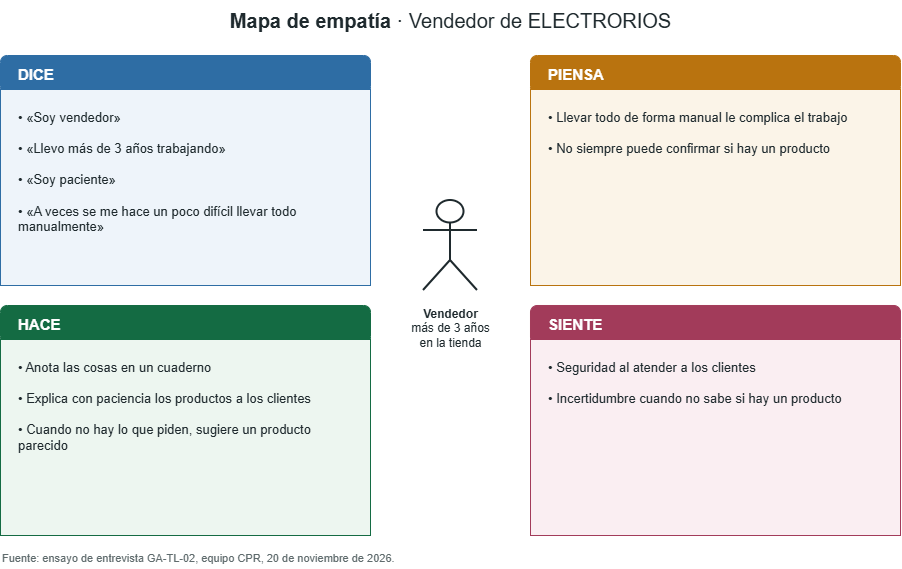
\includegraphics[width=\columnwidth]{figuras/mapa_empatia.png}
\caption{Mapa de empatía de la parte interesada}
\label{fig:empatia}
\end{figure}

\section{Definición del problema}
¿Cómo podríamos ayudar al vendedor a saber si hay un producto disponible para que atienda a los clientes de forma más rápida y fluida?
\par\noindent\begin{minipage}{\columnwidth}
\section{Ajustes al guion}
\centering\scriptsize
\setlength{\tabcolsep}{3pt}
\makeatletter\def\@captype{table}\makeatother
\caption{Preguntas defectuosas detectadas en el ensayo y su corrección}
\label{tab:ajustes}
\begin{tabularx}{\columnwidth}{@{}P{0.5cm}YYY@{}}
\toprule
N.\textordmasculine & Pregunta original & Defecto & Versión corregida\\\midrule
6 & ¿Cómo sabe usted si hay el producto? & La respuesta describió alternativas y dejó sin explicar cómo se verifica el stock. & Cuando un cliente le pide un producto, ¿cómo verifica si hay unidades disponibles? \\
9 & ¿Qué pasa si un cliente quiere devolver un producto que ya compró? & La respuesta indicó que se haría la devolución, pero no explicó cómo se tramita. & Cuando un cliente solicita una devolución, ¿qué pasos sigue usted para tramitarla? \\
\bottomrule
\end{tabularx}
\end{minipage}\par\vspace{4pt}

\section*{Uso de inteligencia artificial}
Se utilizó Claude (Anthropic), modelo Claude Opus 5.5, el 20 de noviembre de 2026,
solo para crear la estructura de carpetas. También se usó para revisar la ortografía y para pasarlas
al formato \LaTeX{}. Las ideas de las preguntas, el ensayo, el mapa de empatía,
la definición del problema y los ajustes son trabajo del equipo.
% Completar: como verifico el equipo lo obtenido (p. ej., compilacion local,
% revision de ISBN en el sitio de la editorial).

\printbibliography
\end{document}
